%%% File: ./inputs/parts/EXECUTIVE_CONTROL.tex

%%% %%%%%%%%%%%%%%%%%%%%%%%%%%%%%% BEGIN PREFRONTAL HIERARCHY %%%%%%%%%%%%%%%%%%%%%%

There is a growing consensus and a fair bit of evidence to support the hypothesis that the human frontal cortex is in charge of executive control, goal-directed planning and abstract thinking. There are differences in opinion about how these cognitive processes are implemented and how they coordinate their activities with that of the rest of the brain. One thing that seems clear is that the frontal cortex and in particular the prefrontal cortex employs many of the same strategies as do networks elsewhere in the brain, both cortical and subcortical.

In particular, circuits in the prefrontal cortex recapitulate the coarse-to-fine, concrete-to-abstract feature hierarchies that we see in the sensory, motor and somatosensory cortex. They exhibit the profuse reciprocal recurrent connections between levels of abstraction that enable us to generalize on the basis of relatively small amounts of information, learn to make accurate predictions in an unsupervised manner depending on observations and interactions with the environment to ground our conclusions, and that provide the foundation for constructing a rich repertoire of representations that serve decision-making.

The neural correlates of abstract thinking, including the circuits that enable us to solve practical problems as well as pursue pure mathematics, are generally agreed to be located in the prefrontal cortex with reciprocal connections throughout the rest of the cerebral cortex, the cerebellar cortex and subcortical regions including the basal ganglia, hippocampal formation and parts of the limbic system involved with emotion, motivation and episodic memory. See {\urlh{box_abstract}{Box~\colorred{C}}} for more detail regarding abstraction, hierarchy and executive oversight in the prefrontal cortex.

%%%%%%%%%%%%%%%%%%%%%%%%%%%%%%%%%%%%%%%%%%%%%%%%%%%%%%%%%%%%%%%%%%%

%%% File: ./inputs/boxes/BOX_EUGENE_LEWIS.tex

\begin{center}
  %%% \begin{tcolorbox}[sharp corners=all,coltitle=black,colbacktitle=white,
  \begin{tcolorbox}[breakable,sharp corners=all,coltitle=black,colbacktitle=white,
    width=\textwidth,boxsep=5pt,left=5pt,right=5pt,
    title={\textbf{Box C: Hierarchy, Abstraction and Executive Control}}]

    %%% width=\textwidth,boxsep=5pt,left=5pt,right=5pt,hypertarget={box_abstract},
    
~~~~The prefrontal cortex (PFC) is generally considered to be responsible for executive cognitive control and enabling the synthesis of novel behavior. Here, we briefly review prefrontal anatomy, development and physiology, focusing on three key executive cognitive functions: {\it{attentional set}}, {\it{working memory}} and {\it{action selection}}. For each function, we suggest how our current understanding might lead to new architectures and algorithms for AI systems.

~~~~The PFC sits atop a group of hierarchically organized sensory and motor areas in the cortex enforced through reciprocal anatomical connections~\cite{FusterPREFRONTAL-CORTEX-15}. This arrangement, referred to as {\it{Fuster’s hierarchy}}, motivates computational models of the PFC that posit the development of highly abstract representations of the sensorimotor context that can be used understand what we perceive and direct how we act~\cite{BotvinickPTRS_B-07}. In addition to connections between layers, Fuster’s hierarchy stipulates reciprocal connections between sensory and motor areas of cortex at the same level of abstraction within each layer of the hierarchy. This intralayer connectivity between perception and motor suggests that action representations feed back into and enhance perception, a principle codified in the notion of {\it{corollary discharge}}~\cite{mccloskey2011corollary}.

~~~~Beyond the model of network interactions, intralayer connectivity in Fuster's hierarchy suggests that each layer of the hierarchy along with the layers below but excluding those above, forms a self-contained perception-action loop. Evidently the neocortex undergoes a series of developmental stages with the PFC among the last areas to mature~\cite{guillery2005postnatal}. This implies training of a complex agent may need to unfold in a manner akin to greedy layer-wise deep network training~\cite{BengioetalNIPS-07,belilovsky2018greedy}, with developmentally-staged, abstraction-comparable, layer-wise learning of the coupled sensorimotor features.

~~~~{\it{Attentional set}} (ASET) refers to the preparation of downstream perception and motor cortices for expected stimuli or action. ASET is exhibited in {\it{cued-attention tasks}} where, in anticipating a visual stimuli, PFC and V4 will be active before the stimuli is given~\cite{sylvester2009anticipatory}. ASET suggests existing inhibitory attention masks may be augmented with additive excitatory attention, allowing a neural network to reduce bottom-up input needed for neuron stimulation or cause neuron firing in the absence of sensory input altogether. Allowing the controller to generate new patterns via network activation even suggests a new model of imagination, with improvements in both sensory synthesis~\cite{GregoretalCoRR-15} and planning~\cite{PascanuetalCoRR-17}.

~~~~{\it{Working memory}} is the maintenance of recent stimuli for subsequent action planning. Working memory consists of groups of coupled neural circuits in the PFC called {\it{stripes}} that are connected to potential target stimuli in sensory cortex and access controlled by circuits in the basal ganglia. Computational models of working memory~\cite{HazyetalPTRS-07} include implementations similar to the recurrent memory circuit of an LSTM cell~\cite{HochreiterandSchmidhuberNC-97}, more exotic architectures involving stacked LSTMs~\cite{graves2013speech} and multiple memory stripes manipulated by a central controller.

~~~~In {\it{action selection}}, the PFC generates many actions that are approved or denied by the basal ganglia; both basal ganglia and orbitomedial PFC receive dopaminergic afferents originating in midbrain structures, providing a reward signal that reinforces learning~\cite{FusterPREFRONTAL-CORTEX-15}. Computational models of dopaminergic systems~\cite{o2007pvlv} point to an architecture similar to existing actor-critic models~\cite{MnihetalCoRR-16}; a key improvement is the modeling of {\it{reward inhibition}}, whereby learning ceases for repetitive stimuli. Suppression of reward to prevent response overfitting could aid in tackling other problems such as reward hacking~\cite{amodei2016concrete}, catastrophic forgetting, and lifelong learning~\cite{ZhiyuanandBingLML-18}, all challenges in effectively managing the learning process.

  \end{tcolorbox}
\end{center}
 

%%%%%%%%%%%%%%%%%%%%%%%%%%%%%%%%%%%%%%%%%%%%%%%%%%%%%%%%%%%%%%%%%%%

With respect to hierarchical goal-based planning, there is growing evidence pointing to a set of adjoining regions in the prefrontal cortex that are responsible for how abstract plans are initially selected, subsequently refined and finally realized as concrete actions. These same regions also appear to be involved in relational reasoning from simple binary relations to higher-order relationships.

These theoretical observations combined with behavioral studies and fMRI recordings have led to a number of computational models of hierarchical planning that exhibit similar patterns of cognitive activity. In particular, cognitive neuroscientists have developed models of how such abstract hierarchical reasoning in the prefrontal cortex is related to what we know about how the basal ganglia and areas of the limbic system involved in motivation contribute to action selection~\cite{OReillySCIENCE-06}. 

%%%%%%%%%%%%%%%%%%%%%%%%%%%%%%%%%%%%%%%%%%%%%%%%%%%%%%%%%%%%%%%%%%%

%%% Figure~{\urlh{#fig_Prefrontal_Hierarchy_Biology_Technology}{\ref{fig_prefer}}
\begin{figure}
%
  \begin{center} 
%    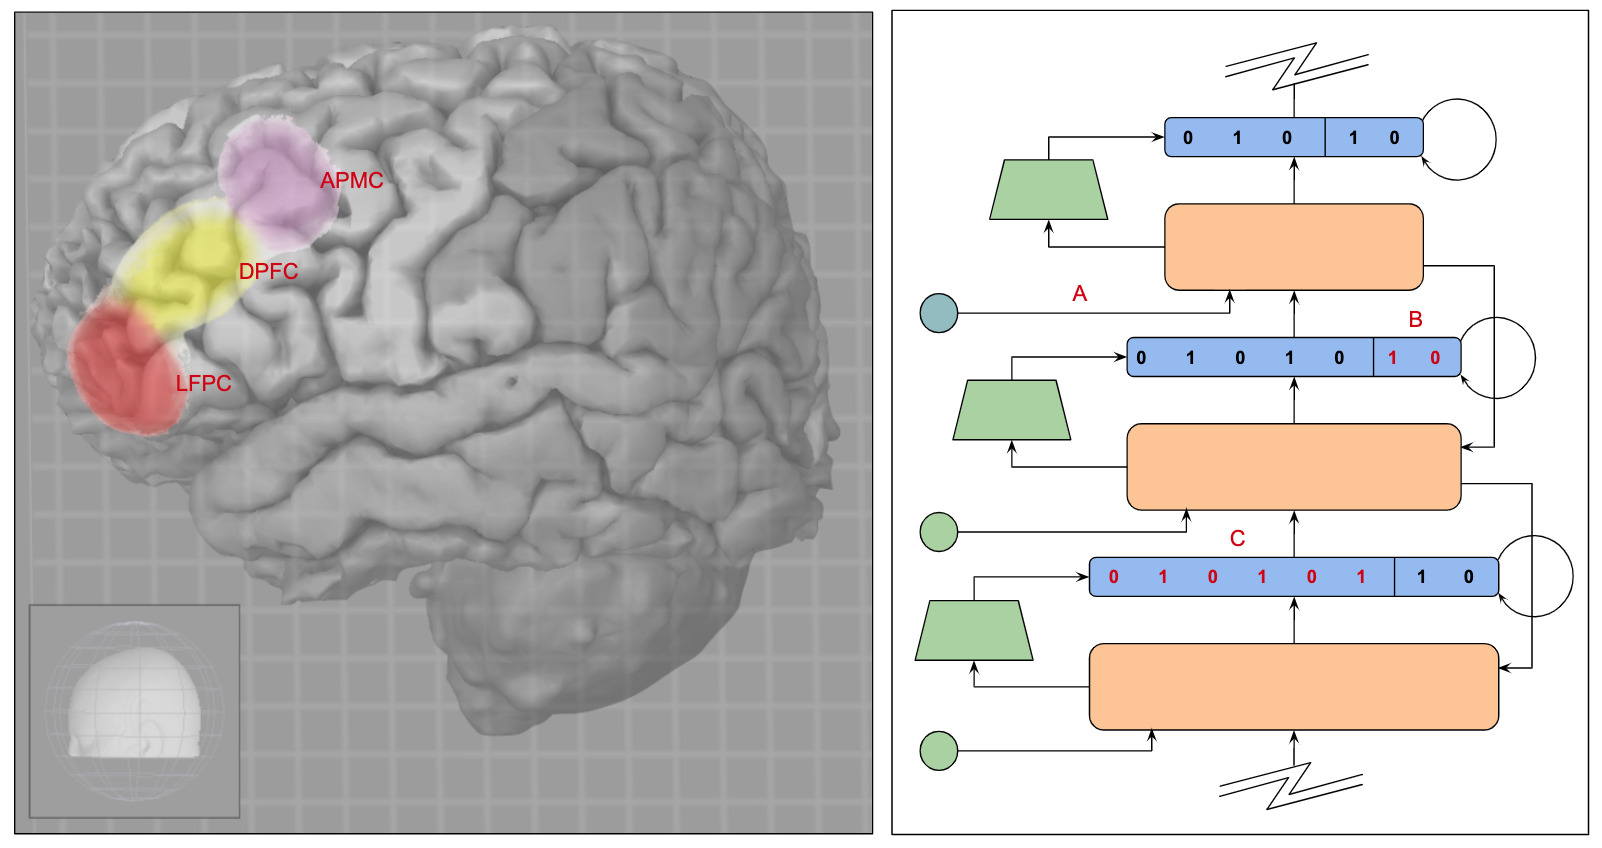
\includegraphics[height=600pt]{./figures/Prefrontal_Hierarchy_Biology_Graze.png} 
    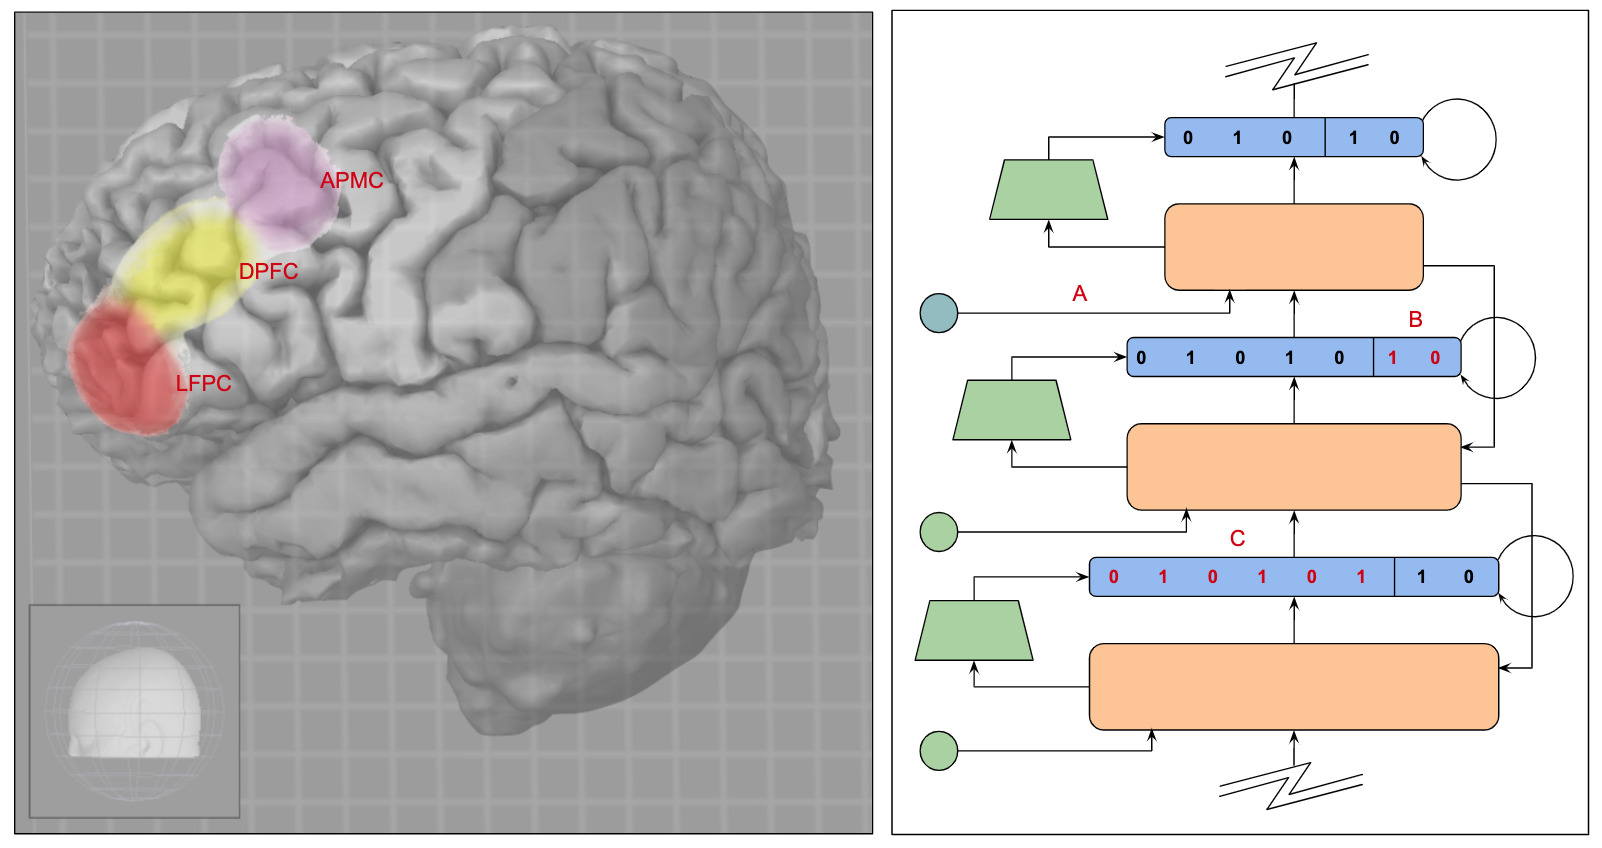
\includegraphics[height=150pt]{./figures/Prefrontal_Hierarchy_Biology_Graze.png} 
  \end{center}
%
  \caption{%
%
    The panel on the left highlights three areas of the prefrontal cortex shown in the figure from left to right (rostro-caudal) and referred to in the text as the {\it{lateral frontal polar cortex}} (\colorred{LFPC}) {\it{dorsolateral prefrontal cortex}} (\colorred{DPFC}) and {\it{anterior premotor cortex}} (\colorred{APMC}). According to the theory first articulated by Joaqu\'{i}n Fuster and subsequently refined David Badre~\cite{BadreandWagnerNEURON-04}, Mark D'Esposito~\cite{DEspositoetalNATURE-95} and Etienne Koechlin~\etal~\cite{KoechlinetalSCIENCE-03} and their colleagues, as actions are specified from abstract plans to concrete responses, progressively posterior regions of lateral frontal cortex are responsible for integrating more concrete information over more proximate time intervals. This process of progressive articulation does not correspond to different stages of execution so much as to how actions are selected, maintained and inhibited at multiple levels of abstraction~\cite{BadreTiCS-08}. The panel on the right shows a simple neural-network model of the brain regions aligned with the rostro-caudal axis of the frontal cortex and hypothesized to account for how action representations are selected, maintained and inhibited at multiple levels of abstraction. The neural-network model is described in more detail in the main text, but a few points are in order here: {\colorred{A}} {\emdash{}} different abstraction layers may include input from other sources, e.g., natural language embeddings, that are only required at particular levels of abstraction; {\colorred{B}} {\emdash{}} each recurrent level of the abstraction hierarchy includes state variables encoding information that would typically appear on the call stack in a conventional computer architecture; {\colorred{C}} {\emdash{}} attentional layers mask (suppress) input that is not determined to be relevant to decision making at a given time and level of abstraction resulting in a sparse context vector.}
%
  \label{fig_prefer}
%
\end{figure}

%%%%%%%%%%%%%%%%%%%%%%%%%%%%%%%%%%%%%%%%%%%%%%%%%%%%%%%%%%%%%%%%%%%

The network shown on the right in Figure~{\urlh{#fig_Prefrontal_Hierarchy_Biology_Technology}{\ref{fig_prefer}}} consists of three subnetworks that roughly align with the {\urlh{https://en.wikipedia.org/wiki/Frontal_lobe}{lateral frontal polar cortex}} (bottom), {\urlh{https://en.wikipedia.org/wiki/Dorsolateral_prefrontal_cortex}{dorsolateral prefrontal cortex}} (middle) and {\urlh{https://en.wikipedia.org/wiki/Premotor_cortex}{anterior premotor cortex}} (top) as shown in the figure. Each of the subnetworks is composed of three elements: a recurrent multilayer perceptron constructed of interleaved convolutional and max-pooling layers shown in orange, a multilayer attention network shown in green and a masking layer in blue that selectively suppresses a subset of the outputs of the convolutional stack in accordance with the output of the attention network.

Input to each of the three subnetworks includes areas of associative activity throughout the sensory and motor cortex as well as areas corresponding to higher-level abstractions located in the frontal cortex responsible for abstract thought and subcortical regions responsible for motivation. While not emphasized here, the active maintenance in working memory of information originating from these sources\footnote{%
  %
  Susan Courtney provides an excellent overview of the many sources of information that are utilized by cognitive functions supported in the frontal cortex~\cite{CourtneyCABN-04}. In particular, her articulation of the role of attention and cognitive control aligns with the views that we've emphasized in class and that drive our designs:
  %
\begin{quotation}
  %
  [The circuits in the prefrontal cortex that drive goal directed planning and executive control] receive multimodal information about the current environment and have access to previously stored memories. The prefrontal cortex's extensive outputs allow for direct control of motor behavior, but they may also influence behavior indirectly by altering perceptual and cognitive representations and influencing the storage and re- trieval of long-term memories.\\
  I suggest that attention and cognitive control are not directed actions or specific processes contained within any particular set of brain regions. Rather, what we experience and observe that we call attention and cognitive control are emergent properties dependent on the dis- tributed representation of all types of information, both that available from present perceptual input and the information currently sustained in WM, including contextual and motivational information.
%
\end{quotation}}
%
is critical for the cognitive activities that these networks support~\cite{CourtneyCABN-04,Goldman-RakicARN-88}. The outputs are fed to a network (not shown) that serves as the interface for the peripheral motor system (the fully instrumented integrated development environment (FIDE) in the case of the programmer's apprentice) which could play the role of the basal ganglia and cerebellum, but could also be considerably simpler depending on the application.

Figure~{\urlh{#fig_Prefrontal_Hierarchy_Biology_Technology}{\ref{fig_prefer}}} is just a sketch employing familiar neural network components to make the point that building these architectures out of standard components is not the most significant challenge. The real challenge is in training them as part of larger system with lots of moving parts. The expectation here, as in the model sketched in Figure~{\urlh{#fig_Hippocampus_Inspired_Learning_Redux}{\ref{fig_hippo}}}, is that end-to-end training with stochastic gradient descent isn't going to work, and that training will likely require some form of layer-by-layer developmentally-staged curriculum learning~\cite{LampinenetalCoRR-19,GulcehreetalCoRR-16,BengioetalCoRR-15,BengioetalICML-09} and a strategy for holding some weights fixed while adjusting other weights to account for new information and avoid problems like catastrophic forgetting.

%%% %%%%%%%%%%%%%%%%%%%%%%%%%%%%%%% END PREFRONTAL HIERARCHY %%%%%%%%%%%%%%%%%%%%%%%
